%!TEX encoding = UTF-8 Unicode
%!TEX TS-program = pdflatex

%%% --- PREAMBLE --- %%%

\documentclass[a4paper,11pt]{article}

\usepackage[italian]{babel}
\usepackage[left=2cm,right=2cm,top=2cm,bottom=2cm]{geometry}
\usepackage[T1]{fontenc} % OT1: basic, T1: western, T3 and T5: exotic, T4: lots of characters but WORSE READABILITY
\usepackage[utf8x]{inputenc} % utf8x supports more characters than utf8
\usepackage{graphicx} % import PNG, JPG and PDF with \includegraphics
\usepackage[usenames,table]{xcolor} % \color
\usepackage{amssymb}
\usepackage{amsmath}
\usepackage{amsfonts}
\usepackage{float}
%\usepackage{mathtools} % (!! PLACE BEFORE hyperref !!)
%\usepackage{xfrac} % \sfrac
%\usepackage{cancel} % \cancel \cancelto
%\usepackage{hyperref} % interactive links in TOC, URLs and references
% unneded \usepackage{fixltx2e} % provides \textsubscript and makes some fixes
%\usepackage[version=3]{mhchem} % \ce (chemical formula)
\usepackage{siunitx} % \num \si \SI
%\usepackage{alltt} % {alltt} (like verbatim but with commands)
%\usepackage{moreverb} % {listing}
\usepackage{listings} % {lstlisting}
%\usepackage[overload]{textcase} % fixes \MakeUppercase and \MakeLowercase
%\usepackage[normalem]{ulem} % \uline \uwave \sout \xout
%\usepackage{enumerate} % adds options for {enumerate}
%\usepackage{paralist} % inline lists with {inparaenum}
%\usepackage[official]{eurosym} % \euro
%\usepackage{tabu} % {tabu} (like {tabular} with improvements)
%\usepackage{layout} % layout description
\usepackage{multicol} % {multicols}
%\usepackage{lipsum} % filling text generator with \lipsum
%\usepackage[section]{placeins} % inhibits float figures from trepassing a section boundary
\usepackage{subfig} % \subfloat to be used inside {figure}
%\usepackage{wrapfig} % {wrapfigure} (like {figure} but allows text to flow on its sides)
%\usepackage{ifthen} % \ifthenelse
%\usepackage{calc}
%\usepackage{array}
\usepackage{multirow}
\usepackage{booktabs} % \toprule, \midrule, \bottomrule

\graphicspath{ {../Figs-Tabs/} } % graphics search directories
\setcounter{tocdepth}{1} % -1: part, 0: chapter, 1: section, 2: subsection, 3: subsubsection

\lstset{ %
	language=C,
	deletekeywords={},
	morekeywords={},
	backgroundcolor=\color{white},
	basicstyle=\ttfamily\small,
	commentstyle=\color{teal},
	keywordstyle=\color{magenta},
	stringstyle=\color{purple},
	identifierstyle=\color{violet!80!black},
	numbers=left,
	numbersep=7pt,
	numberstyle=\scriptsize\sffamily\color{gray},
	stepnumber=1,
	breakatwhitespace=false,
	breaklines=true,
	keepspaces=true,
	showspaces=false,
	showstringspaces=false,
	showtabs=false,
	tabsize=2,
	captionpos=none,
}

\newcommand{\swaphmargins}{
\newlength{\tmplength}
\setlength{\tmplength}{\oddsidemargin}
\setlength{\oddsidemargin}{\evensidemargin}
\setlength{\evensidemargin}{\tmplength}}

\newcommand{\setdispacing}[1][0pt]{\setlength{\abovedisplayskip}{#1}
\setlength{\belowdisplayskip}{#1}
\setlength{\abovedisplayshortskip}{#1}
\setlength{\belowdisplayshortskip}{#1}}

\newcommand{\inv}[1]{\frac{1}{#1}}
\newcommand{\dd}{\mathrm{d}}
\newcommand{\deriv}[2][x]{\frac{\dd #2}{\dd #1}}
\newcommand{\derivn}[3][x]{\frac{\dd^{#2}#3}{\dd{#1}^{#2}}}
\newcommand{\pardv}[2][x]{\frac{\partial #2}{\partial #1}}
\newcommand{\pardvn}[3][x]{\frac{\partial^{#2}#3}{\partial{#1}^{#2}}}
\newcommand{\integ}[2][x]{\int #2\,\dd #1}
\newcommand{\invinteg}[2][x]{\int\frac{\dd #1}{#2}}
\newcommand{\dinteg}[4]{\int_{#1}^{#2}#3\,\dd #4}
%\renewcommand{\arcsin}{\operatorname{asin}}
%\renewcommand{\arccos}{\operatorname{acos}}
%\renewcommand{\arctan}{\operatorname{atan}}
\DeclareMathOperator{\arccot}{arccot}
\newcommand{\vel}{\vee}
\newcommand{\et}{\wedge}

\newcommand{\fwhm}{\text{FWHM}}
\newcommand{\hwhm}{\text{HWHM}}

\newcommand{\ndr}[1]{\footnote{#1 (n.d.r.)}}
\newcommand{\fig}[1]{figura (\ref{f:#1})} %inserting reference to figures
\newcommand{\tab}[1]{tabella (\ref{t:#1})} % inserting reference to tables
\newcommand{\dof}{\text{ dof}} % degrees of freedom
\newcommand{\paral}{\mathbin{\|}} % impedance parallel
\DeclareSIUnit\deca{decade} % decade unit definition for use in siunitx

\newcommand{\insertpart}[2]{\input{#1}}

\sisetup{%
	separate-uncertainty = true,
	per-mode = symbol,
	bracket-numbers = false,
	multi-part-units = single,
	table-number-alignment = center,
	range-phrase = \text{--},
	range-units = brackets,
	output-complex-root =  \text{\ensuremath{j}},
	table-figures-decimal = 3,
	table-figures-exponent = 0,
	table-figures-integer = 2,
	table-figures-uncertainty = 2,
}

%%% --- DOCUMENT --- %%%


%%%%% SIunitX example use:
% \si{\kilo\volt\per\meter\squared} -> kV/m^2
% \SI{1.222 (34)}{\joule\second}    -> 1.222 +- 0.034 Js
% \SI{1.222 \pm 0.034}{\nF}         -> 1.222 +- 0.034 nF
% use it plz

\author{Gruppo BF \\ Thomas Giannoni, Valerio Lomanto, Roberto Ribatti}
\title{Esperienza N.3 Franck-Hertz.}
\date{2 marzo 2017}

\begin{document}
	\maketitle
	\begin{abstract}
		In quest'esperienza si è analizzata la natura quantistica dei 
		livelli energetici dell'atomo di Neon e si é stimato il gap di energia 
		tra il livello fondamentale ed il primo eccitato. Ai fini di tale studio si sono osservati gli effetti 
		dissipativi degli urti anelastici tra elettroni e atomi di
		neon.
	\end{abstract}
%	\tableofcontents %dovrebbe fare l'indice
	\section{Strumentazione}
	In questa esperienza si sono impiegati:
	\begin{itemize}
	\item un tetrodo a gas neon ELWE U84822330;
	\item un sistema di alimentazione e lettura di corrente ELWE;
	\item un oscilloscopio.
	\end{itemize}

Il tetrodo a gas è un tubo contenente Neon a bassa pressione in cui sono disposti 4 elettrodi che nel seguito chiameremo catodo, griglia di controllo, griglia d'anodo e collettore la cui funzione sarà  chiarita in seguito.
L'apparato fornisce la misura dei seguenti parametri:
\begin{itemize}
	\item $U_F\quad$	la d.d.p. applicata ai capi del filamento del catodo;
	\item $U_G\quad$	la d.d.p. tra catodo e griglia di controllo;
	\item $U_G\quad$	la d.d.p. tra catodo e griglia d'anodo;
	\item $U_E\quad$	la d.d.p. tra griglia d'anodo e collettore.
\end{itemize}

Si riporta in \figurename{ \ref{fig:apparato}} uno schema
	dell'apparato sperimentale impiegato.
	\begin{figure} [!h]
		\centering
		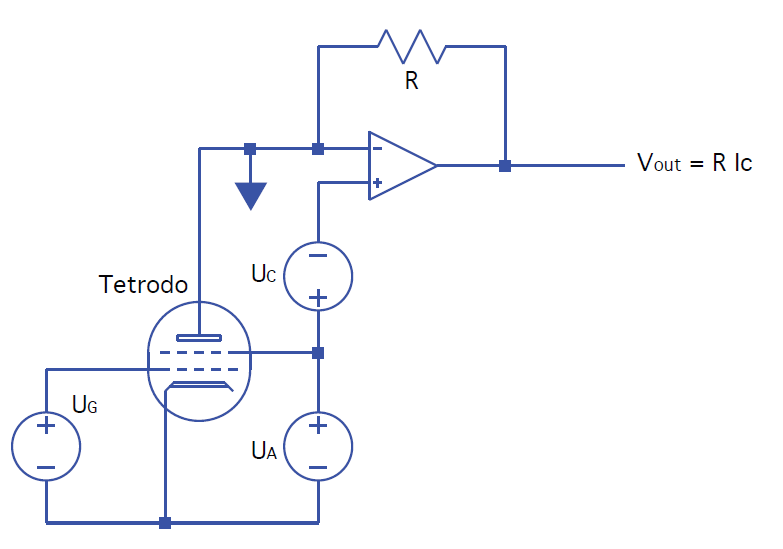
\includegraphics[width=0.5\textwidth]{apparato.png}
		\caption{Schema dell'apparato impiegato.}
		\label{fig:apparato}
	\end{figure}

	\section{Procedura operativa e svolgimento}
	Si � acceso il tetrodo regolando la tensione $U_F$ = \SI{8.0 \pm 0.1}{\volt}
	in modo da innescare la produzione di $e^{-}$ al catodo per effetto 
	termoionico.
	Si � regolato un campo accelerante $U_A=$ \SI{70 \pm 0.1}{\volt}
	dopodich� si � posta una tensione $U_G$ crescente sino a che gli 
	$e^{-}$ raccolti siam stati  sufficienti a produrre n evidenza dalla 
	diseccitazione degli atomi di neon nel tetrodo, righe di colore
	arancione.
	
	Gli elettroni risultano accelerati dalla ddp $U_A-U_G$
	si ottiene pertanto un energia $e^{-} \cdot (U_A-U_G)$.
	si � osservato che aumentando la tensione $U_A$ si ottiene
	d'apprima lo spostamento della riga colorata verso il catodo,
	e successivamente all'ulteriore aumento  della tensione si
	osservano la comparsa di altre righe colorate vicino al anodo.
	
	\begin{table}[hb]
 		\centering
		\begin{tabular}{|c|c|c|}
 			\toprule
 			Ordine  & $U_A$ di apparizione & $U_A- U_G$\\
  			\midrule
  			$1$ & \SI{21.0 \pm 0.5}{\volt} &\SI{16.2 \pm 0.6}{\volt}\\
  			$2$ &  \SI{36.5 \pm 0.5}{\volt} &\SI{32.1 \pm 0.6}{\volt}\\
  			$2$ &  \SI{57.0 \pm 0.5}{\volt} &\SI{53.5 \pm 0.6}{\volt}\\
  			\bottomrule
 		\end{tabular}
 	\caption{$U_A$ corrispondenti all'apparizione delle righe 
 			colorate vicino all'anodo.
 			Si segnala che a causa dell'illuminazione ambientale
 			l'individuazione della comparsa della riga potrebbe essere stata
 			individuata con un ritardo,con conseguente sovrastima delle
 			tensioni necessarie.}
	\label{tab:a}
	\end{table}
	Si riportano le tensioni di apparizione di tali righe in \tab{tab:a}.
	
	Questo andamento � da imputarsi al fatto che il trasferimento 
	di energia negli urti tra $e^{-}$ e gli atomi di He sia 
	quantizzato. Gli elettroni possono eccitare gli atomi di
	He, esclusivamente quando hanno un energia maggiore o uguale
	al gap energetico tra i livelli eccitati ed il fondamentale.
	Essendo l'energia degli $e^{-}$ proporzionale alla distanza 
	percorsa nel tetrodo ed alla d.d.p. $U_A-U_G$,
	alla crescita della tensione $U_A$ si riduce
	la distanza necessaria per ottenere l'energia necessaria 
	per l'eccitazione del He; pertanto la striscia 
	dovuta alla diseccitazione si sposta verso il catodo.
	
	All'ulteriore aumento del campo accelerante dopo il
	primo urto,e conseguentemente all'eccitazione degli 
	atomi di neon, gli elettroni acquisiscono un energia
	sufficiente per rieccitare gli atomi 
	di neon in un tratto successivo del tetrodo ;
	a ci� corrisponde la comparsa delle ulteriori righe colorate.
	
	Si osserva inoltre che all'aumentare di $U_G$ le righe risultano
	pi� intense.	 
	Questo effetto risulta compatibile col fatto
	che la tensione $U_G$ regola la tensione della griglia di controllo,
	e conseguentemente all'aumentare di $U_G$ aumenta il numero di elettroni
	che vengono raccolti e immessi nel tetrodo, 
	quindi un aumento de il numero di urti che hanno 
	l'energia sufficiente per 	eccitare gli atomi di Ne.
	
	Si � settato apparato strumentale in modo che
	la tensione $U_A$ sia in modalit� rampa;tra 0 e il suo massimo 
	(\SI{80.0 \pm 0.5}{\volt}).
	Attraverso la modalit� X-Y dell'oscilloscopio si � 
	osservato l'andamento della curva $I_C$ $VS$  $U_A$
	variare di $U_E$.
	
\begin{figure}[!h]
		\centering
		 \subfloat[$U_E=$\SI{1.0 \pm 0.1}{\volt}]{
		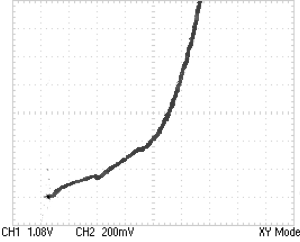
\includegraphics[scale=0.5]{./fig/ue1.png}
		\label{f:ue1}
		}
		 \subfloat[$U_E=$\SI{3.0 \pm 0.1}{\volt}]{
		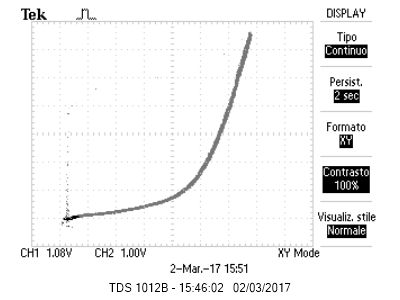
\includegraphics[scale=0.5]{./fig/ue3.png}
		\label{f:ue3} 
		}//
		 \subfloat[$U_E=$\SI{3.4 \pm 0.1}{\volt}]{
		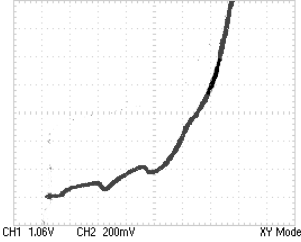
\includegraphics[scale=0.5]{./fig/ue34.png}
		\label{f:ue3.4}
		}
		 \subfloat[$U_E=$\SI{7.5 \pm 0.1}{\volt}]{
		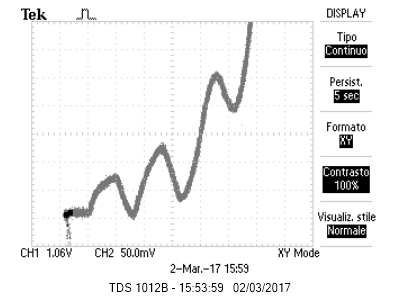
\includegraphics[scale=0.5]{./fig/ue75.png}
		\label{f:ue7.5}
		}
		\caption{$I_C$ vs $U_A$ al variare di $U_E$ in modalit� X-Y}
	\label{fig:ue}
\end{figure}
	Si riportano gli andamenti osservati in \fig{fig:ue}.
	Come � possibile osservare dalle \fig{f:ue1} e \fig{f:ue3}
	per valori del campo decelerante $U_E-U_A$ 
	bassi la quasi totalit� degli $e^{-}$, anche qualora facciano
	urti elastici, raggiunge il collettore dando luogo alla corrente $I_C$.
	Aumentando $U_E$ si osserva un decremento 
	di $I_C$;ci� risulta compatibile col fatto che gli $e^{-}$
	dopo aver ceduto energia per l'eccitazione degli atomi di He
	non hanno l'energia per superare il campo di decelerazione. 
	Tale andamento pone in evidenza la struttura classica della
	curva di Franck-Hartz \fig{f:ue7.5}.
	
	Dalla regolazione di $U_E$ si sono settati i minimi della curva 
	$I_C VS U_A$ in corrispondenza dello zero.
	Si � regolato il valore di $U_A$ in maniera da osservare il massimo
	numero di massimi osservabili sullo schermo dell'oscilloscopio,
	� stato inoltre necessario regolare il guadagno dell'amplificatore
	in maniera da non saturare.
	A seguito si � disinserita la modalit� X-Y dell'oscilloscopio 
	e si sono acquisite le due tracce di $U_A$ e $I_C$ al variare di 
	$U_E$ da $11 V$ a $0V$. Per  tali acquisizioni,qualora non si siano 
	verificati problemi a rilevare i picchi, sono stati 
	osservate le $U_A$ corrispondenti ai massimi di $I_C$.
	-FORSE CONVIENE TABLARLI CHE DITE?-
	Con tali dati si � eseguito n fit lineare 
	-RIPORTARE FIT-
	ottenendo come valori dei picchi
	$ U_{A_1,max}=$ \SI{ \pm 0.}{\volt} $ U_{A_2,max}=$ \SI{ \pm 0.}{\volt}
	$ U_{A_,max}=$ \SI{ \pm 0.}{\volt}.
	Si riporta il fit in \fig{fit.png}.
	
	Si osserva che dati sono in accordo con quelli trovati alla 
	verifica qualitativa della comparsa delle frange.
	Si nota inoltre che tali picchi sono presentano un  andamento periodico
	in energia;con una periodo di \SI{ \pm 0.}{\electronvolt}.
	Si � associato tale gap energetico alla differenza di energia 
	tra lo stato fondamentale degli atomi di He e il primo stato eccitato.




\end{document}
